% preamble and style file for M&R lecture slides
\documentclass[11.5pt,sans,english]{beamer}

\usetheme{EastLansing}
\usecolortheme{lily}

\usepackage[most]{tcolorbox}

\usepackage{verbatim}
%\usepackage{ulem}
%\usepackage{fontawesome}
%\usepackage{tikz}
%\usepackage{pifont}
%\usepackage{tabularx}
\usepackage{array,booktabs,xcolor,colortbl,multirow,rotating,amssymb}
%\usepackage{amsmath}
% \usepackage{vwcol}
% \usepackage[T1]{fontenc}

  
\newcommand\vect[1]{\underline{\mathbf{#1}}}
\newcommand\unitvect[1]{\hat{\boldsymbol{#1}}}
%\newcommand\hatdot[1] { \hat{ \dot{ \boldsymbol{#1} } } }

\newtcbox
{\keyc}{on line,arc=2pt, colback=yellow!30!white, colframe=yellow!30!black, before upper={\rule[-3pt]{0pt}{10pt} },boxrule=1pt,boxsep=0pt,left=6pt,right=6pt,top=2pt,bottom=2pt,}

\newtcbox
{\keyb}{on line,arc=1pt, colback=blue!30!white, colframe=blue!30!black, before upper={\rule[-3pt]{0pt}{10pt} },boxrule=1pt,boxsep=0pt,left=6pt,right=6pt,top=2pt,bottom=2pt,}

\newtcbox
{\keyl}{on line,arc=1pt, colback=pink!30!white, colframe=blue!30!black, before upper={\rule[-3pt]{0pt}{10pt} },boxrule=1pt,boxsep=0pt,left=6pt,right=6pt,top=2pt,bottom=2pt,}

\newtcbox
{\keyw}{on line,arc=1pt, colback=red!30!white, colframe=blue!30!black, before upper={\rule[-3pt]{0pt}{10pt} },boxrule=1pt,boxsep=0pt,left=6pt,right=6pt,top=2pt,bottom=2pt,}

\newtcbox
{\keya}{on line,arc=1pt, colback=purple!30!white, colframe=blue!30!black, before upper={\rule[-3pt]{0pt}{10pt} },boxrule=1pt,boxsep=0pt,left=6pt,right=6pt,top=2pt,bottom=2pt,}

\newtcbox[auto counter,number within=section]
{keyf}
{
enhanced,
on line,
  boxsep=0pt,
  left=6pt,right=6pt,top=2pt,bottom=2pt,
  arc=5pt,
  boxrule=1pt,
  rightrule=38pt,
colback=green!10!white, 
colframe=green!50!black, 
title=\thetcbcounter,
detach title,
overlay unbroken and first ={
    \node[%rotate=90,
          %minimum width=1cm,
          anchor=south,
          font=\sffamily\bfseries\tiny,
          %yshift=-10pt,
          yshift=-5pt,
          xshift=-20pt,
          white]
    at (frame.east) {\thetcbcounter};
  }
}


\usepackage{xcolor}

%\usepackage{hyperref}
%\hypersetup{
%  pdfauthor={Lily Asquith},
%  urlcolor=blue,
%  colorlinks=true,
%  linkcolor=blue,
%  bookmarks=true
%}

%---------------------------------------------%
%              LILY'S COLOURS           %
%---------------------------------------------%
\definecolor{Wash}{RGB}{204,204,204}
%\definecolor{Pinky}{RGB}{254,200,254}%violet
\definecolor{Pinky}{RGB}{219,	240,	253}%violet
\definecolor{Bluey}{RGB}{0,190,255}%deep sky blue
\definecolor{DarkGrey}{RGB}{28,66,137}%dar grey
\definecolor{SussexWhite}{RGB}{253,255,254}%dar grey
\definecolor{LightGray}{RGB}{184,184,255}
\definecolor{YesGreen}{RGB}{0,128,0}
\definecolor{NoRed}{RGB}{250,0,0}



\definecolor{myred}{RGB}{255,153,153}
\definecolor{myorange}{RGB}{255,204,153}
\definecolor{myyellow}{RGB}{255,255,153}
\definecolor{mygreen}{RGB}{153,255,153}
\definecolor{mycyan}{RGB}{153,255,255}
\definecolor{myblue}{RGB}{153,204,255}
\definecolor{myviolet}{RGB}{153,153,255}
\definecolor{mypurple}{RGB}{204,153,255}
\definecolor{mypink}{RGB}{255,204,255}
\definecolor{mycoral}{RGB}{255,153,204}

%-----------------------------------------------------%
%              LILY'S COLUMN TYPES          %
%-----------------------------------------------------%
\newcolumntype{a}{>{\raggedright\arraybackslash}l}	
\newcolumntype{q}{>{\raggedright\arraybackslash}m{8cm}} 

%--------------------------------------------%
%              LILY'S SYMBOLS          %
%--------------------------------------------%
\newcommand{\dfinger}{\large{\textcolor{black}{\ding{43}}}\scriptsize}
\newcommand{\dstar}{\large{\textcolor{black}{\ding{76}}}\scriptsize}
\newcommand{\dwrite}{\large{\textcolor{black}{\ding{45}}}\scriptsize}
\newcommand{\ddiamond}{\small{\textcolor{DarkGrey}{\ding{117}}}\scriptsize}
\newcommand{\ddiamondwhite}{\small{\textcolor{SussexWhite}{\ding{117}}}\scriptsize}
\newcommand{\experiment}{\small{\textcolor{magenta}{\faCogs }}\scriptsize}
\newcommand{\watchit}{\textcolor{blue}{ \faYoutube}}


\makeatletter
\newcommand\notsotiny{\@setfontsize\notsotiny{6.5}{7.5}}
\makeatother


% 
\title[ Intro to Quantum Physics]{Intro to Quantum Physics F3241}
%\subtitle{\textbf{Part 2: The Electron}}
\author[Dr Lily Asquith (Lily)]{ Dr Lily Asquith (Lily)}
\date[Week 2]{ Week 2, Lecture 2}
\logo{

\includegraphics[width=1.5cm]{../../utils/uslogo.jpg}
}


\begin{document}


\begin{frame}
\titlepage
\end{frame} 

 %-----------------------------------------------------------%
 % 1 Kinematics                                                 %
 %-----------------------------------------------------------%
\section{I2Q Part 2: The Electron}

 
 %-----------------------------------------------------------%
 % LECTURE 1
 %-----------------------------------------------------------%
 


\begin{frame}{An example problem - part 1: dimensional analysis}
\small
We accelerate a mixed beam of electrons and protons to $3 \times 10^7$ ms$^{-1}$, and allow them to enter a region with a uniform magnetic field perpendicular to their direction with a strength of 8T. What happens to the particles?\\[21ex]

%I will use $F=qvB$, so dimensionally $MLT^{-2} = IT LT^{-1}$ [x unknown Tesla dimension]\\
%%unknown Tesla dimension  = $MLT^{-2} I^{-1}T^{-1} L^{-1}T$ \\
%unknown Tesla dimension  = $MT^{-2} I^{-1}$ \\[1ex]
%Units $T = kg s^{-2} A^{-1} = kg s^{-1} C^{-1}$\\[1ex]
%
%
%
%mass of electron = $9.11 \times 10^{-31}$ kg\\[1ex]
%mass of proton = damn it can't remember, but i do remember it is about 2000 times the mass of the electron \\[1ex]
\end{frame}

\begin{frame}{An example problem - part 2: physics }
\small
We accelerate a mixed beam of electrons and protons to $3 \times 10^7$ ms$^{-1}$, and allow them to enter a region with a uniform magnetic field perpendicular to their direction with a strength of 8T. What happens to the particles?\\[21ex]

%I will use $F=qvB$, so dimensionally $MLT^{-2} = IT LT^{-1}$ [x unknown Tesla dimension]\\
%%unknown Tesla dimension  = $MLT^{-2} I^{-1}T^{-1} L^{-1}T$ \\
%unknown Tesla dimension  = $MT^{-2} I^{-1}$ \\[1ex]
%Units $T = kg s^{-2} A^{-1} = kg s^{-1} C^{-1}$\\[1ex]
%
%
%
%mass of electron = $9.11 \times 10^{-31}$ kg\\[1ex]
%mass of proton = damn it can't remember, but i do remember it is about 2000 times the mass of the electron \\[1ex]
\end{frame}


\begin{frame}{A Quick Recap}

\small
A Volt is a measure of "energy per charge" \\[1ex]
So, energy is "charge times voltage"\\[1ex]
Often this is written "Joules = Coulombs  times Volts" \\[1ex]
When dealing with electrons, we can use " electronVolts = elementary charge times Volts"\\[2ex]

Electric field strength is "voltage per distance"\\[1ex]
Electric force is "charge times Field strength " or " charge times voltage per distance" or "energy per distance"\\[1ex]

\begin{center}
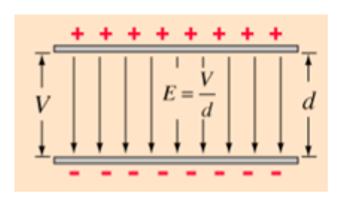
\includegraphics[scale=0.5]{millikan2}
\end{center}
\end{frame}

%-----------------------------------------------------
%     LECTURE 2
%-----------------------------------------------------
%
\subsection{Thomson's Experiment: Bendy Rays}




\begin{frame}{Thomson's Cathode Ray Experiment}
\small
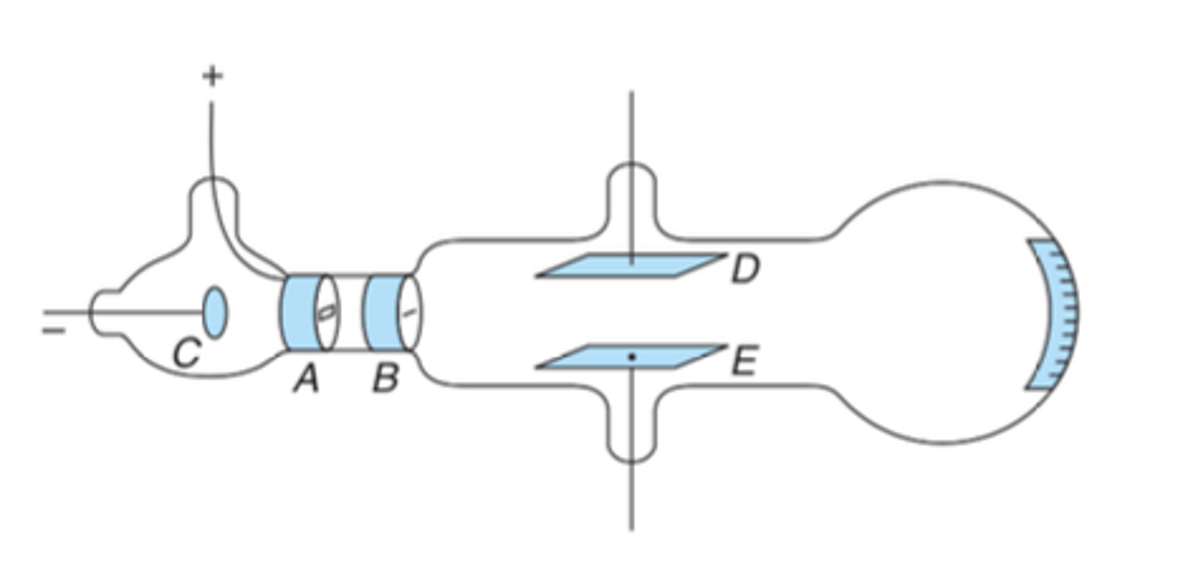
\includegraphics[scale=0.4]{cathode1}
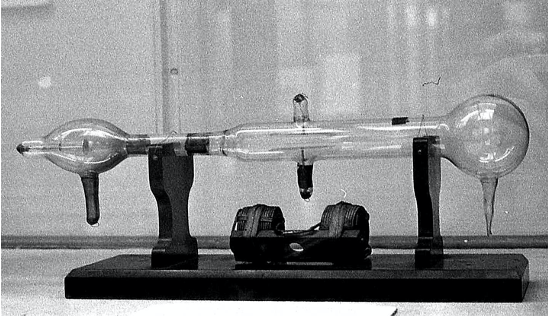
\includegraphics[scale=0.4]{cathode2}
\end{frame}



\begin{frame}{Thomson's Cathode Ray Experiment}
\small
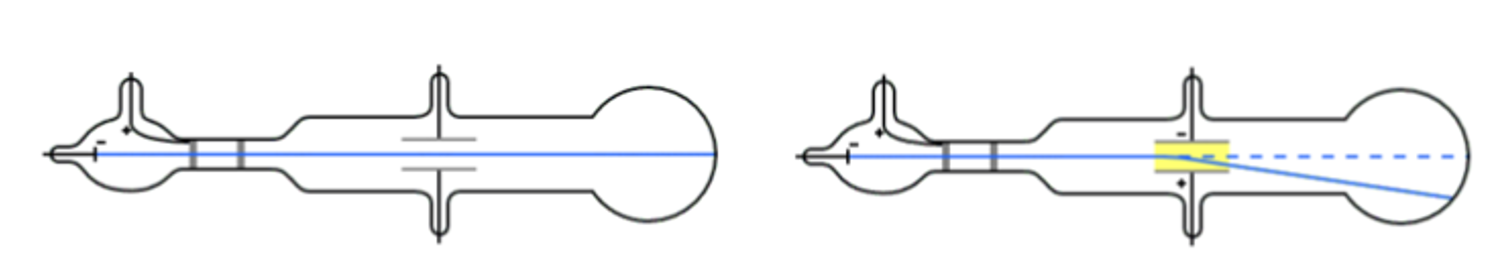
\includegraphics[scale=0.4]{cathode3}

The cathode ray bends towards the + plate when the electric (or magnetic) field is turned on: \\[3ex]

\textbf{Cathode rays are negatively charged.}\\
If cathode rays are made of particles, we can write:\\[4ex]

What can we control in this experiment?\\[2ex]
What can we measure directly?\\[2ex]
What can we measure indirectly?\\[2ex]

\end{frame}



\begin{frame}{Thomson's Cathode Ray Experiment}
\small
What variations of this experiment could tell us more?\\[20ex]

\end{frame}


\begin{frame}{An example problem}
\small
Electrons have kinetic energy of 2000 eV, and are travelling in a CRT with a region of electric field $E = 3.33 \times 10^3$ Vm$^{-1}$. The mass of an electron is 511 keV. \\[2ex]

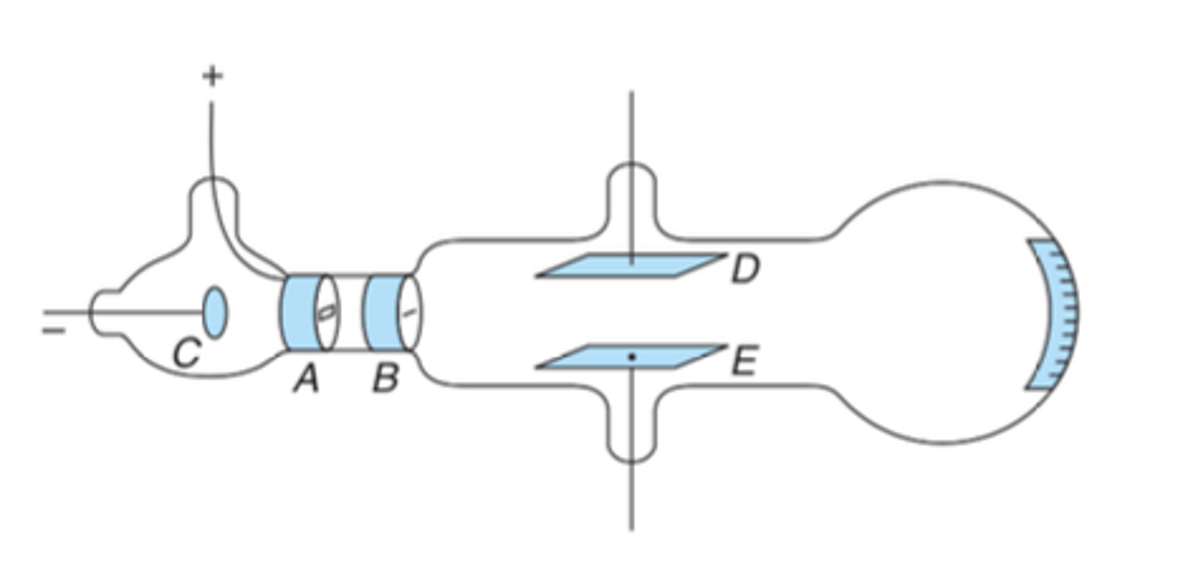
\includegraphics[scale=0.2]{cathode1}



a) What is their speed?\\[18ex]

% note that we are given energy and mass in eV, (c2)
% energy is 2000
% mass is 511,000/c^2 
% KE = 0.5 m v^2, so v = sqrt(2E/m) = sqrt(4e3 / 511e3) 

\end{frame}

\begin{frame}{An example problem}
\small
Electrons have kinetic energy of 2000 eV, and are travelling in a CRT with a region of electric field $E = 3.33 \times 10^3$ Vm$^{-1}$. $m_e$ = 511 keV.\\[2ex]

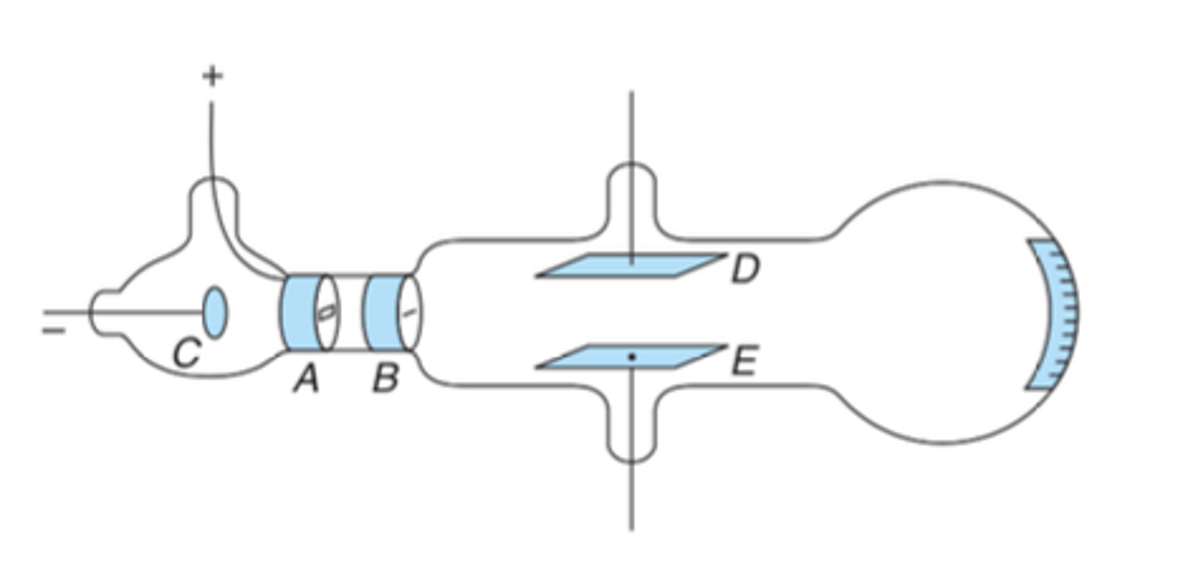
\includegraphics[scale=0.2]{cathode1}


b) What is the time needed to traverse 5 cm  in the region of electric field?\\[18ex]

% note that now they are being accelerated by F_E = qE = Coulombs x Volts per metre = IT
% s =ut  + 0.5at^2
% a = F/m = qE/m = e 3.3 V/m / 511 keV

\end{frame}






%-----------------------------------------------------
%     LECTURE 3
%-----------------------------------------------------

\subsection{Millikan's Experiment: Balancing forces}

\begin{frame}{Millikan's oil drop experiment}
\small
From Thomson's experiment we know $\frac{q}{m}$, but we don't know $q$ or $m$\\[3ex]

Thomson balanced the electric and magnetic forces to extract this ratio.\\[3ex]

\textbf{Millikan had the idea to balance the electric force against the gravitational force.}\\[6ex]
\end{frame}


\begin{frame}{Millikan's oil drop experiment}
\small

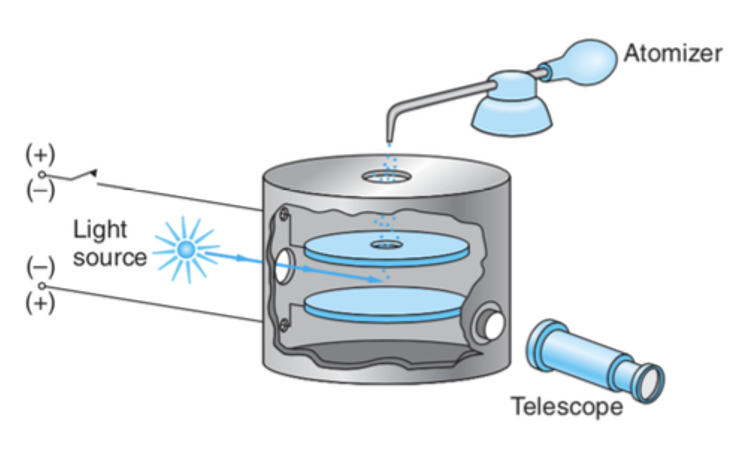
\includegraphics[scale=0.5]{millikan1}

\end{frame}

\begin{frame}{Millikan's oil drop experiment}
\small
What important things did we ignore when going through Millikan's experiment?\\[20ex]
\end{frame}



\begin{frame}{Millikan's oil drop experiment}
\small
\begin{center}
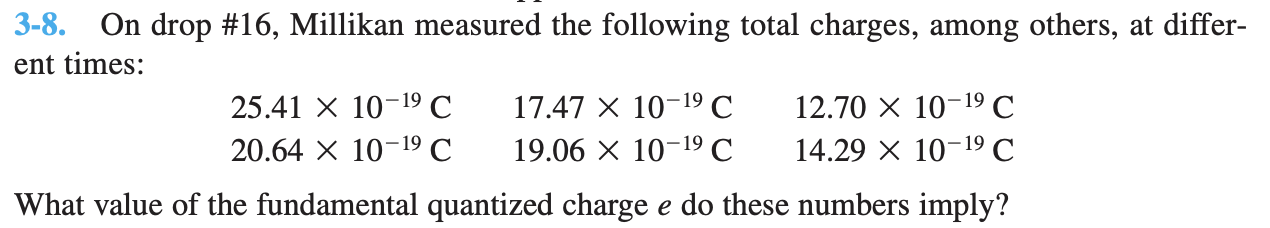
\includegraphics[scale=0.5]{millikan-q}
\end{center}
\vspace{5cm}
\end{frame}







\begin{frame}{Where we are}
\small
\begin{center}
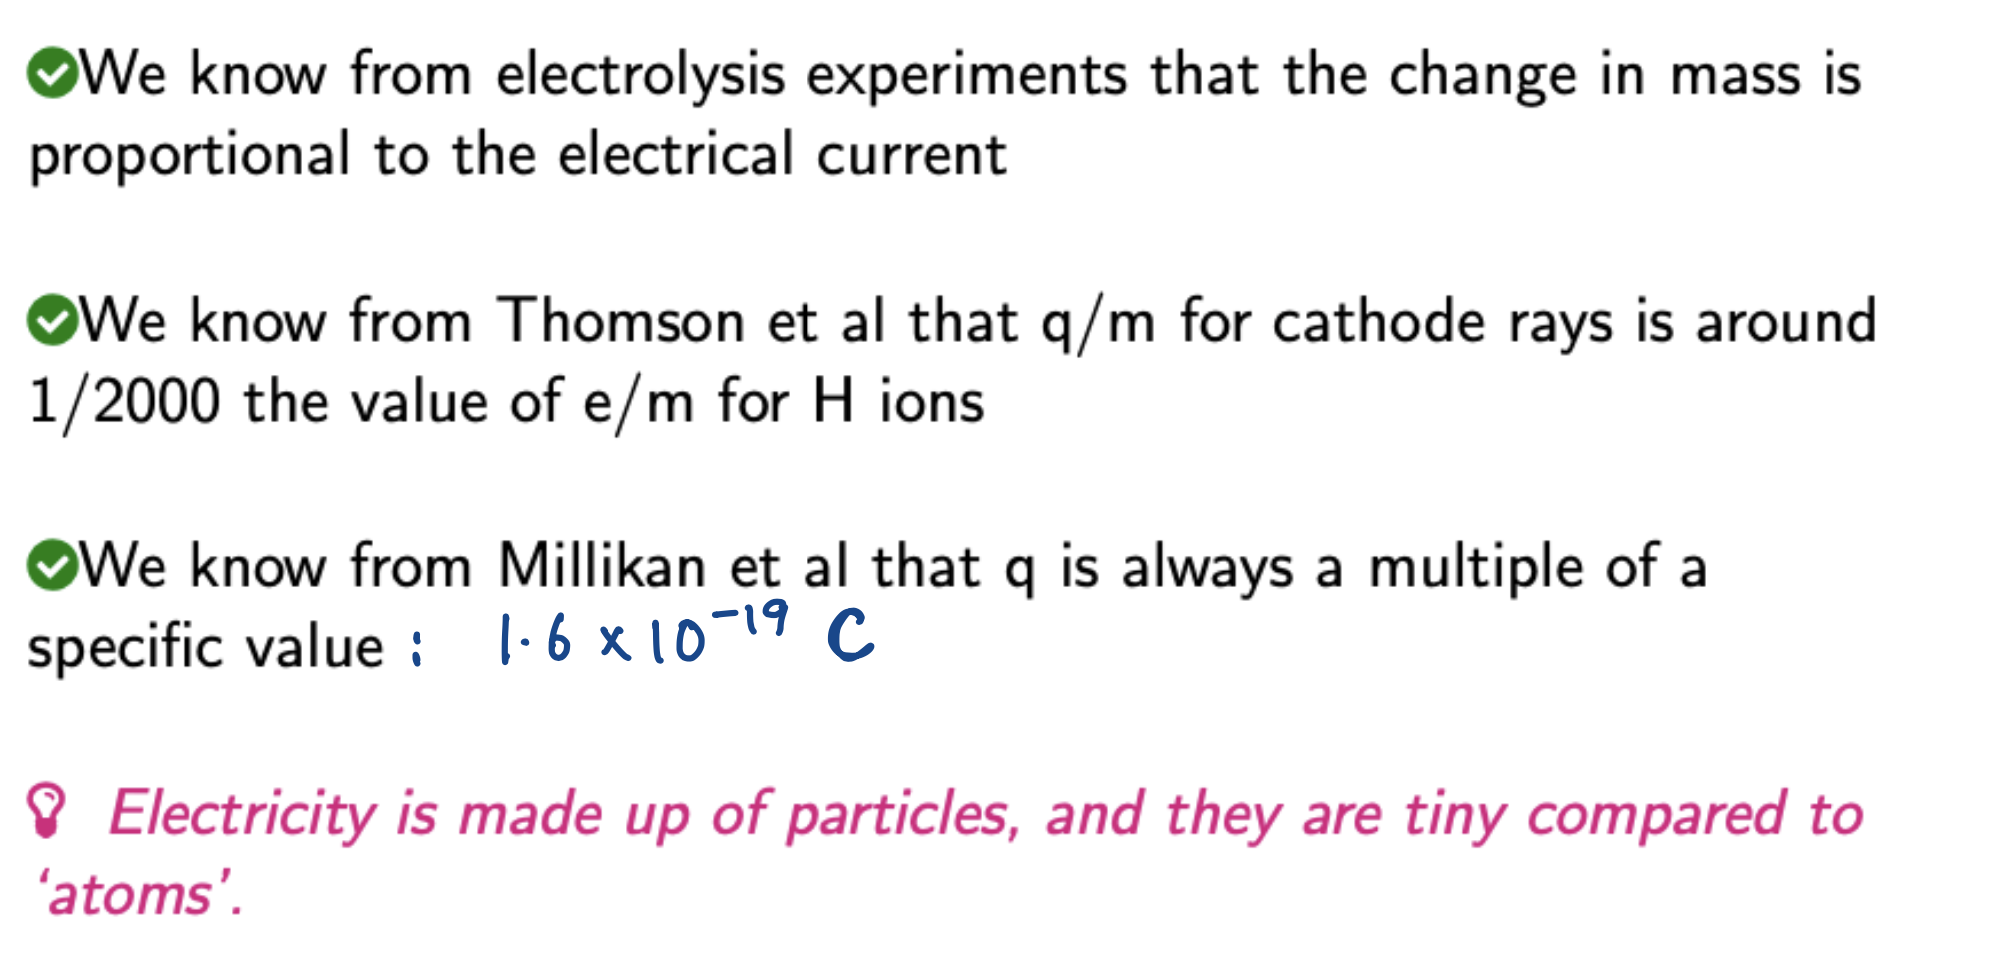
\includegraphics[scale=0.25]{summary}
\end{center}
\end{frame}


 
\end{document}